\chapter{Implementation}
This chapter includes the implementation of controllers and components. The chapter will be seperated into two section, a section for the inverted pendulum and another section for the rocket. An Arduino will be used as the platform to implement the hardware and software on.    


\subsection{MCU}\label{sec:MCU}
TBD

\todo{Sampling speed for both system, and argument that the arduino is fine with its 16 MHz clock speed.}

\section{Inverted Pendulum Implementation}
This section describes the hardware and software implementation of the controllers designed cf. section \ref{sec:IPController}. The goal is to determine if the designed controllers will balance the stick in the real world application. The section is separated into three different parts about sensors, hardware controller and software controller. The first part is to implement the feedback for the controllers which in the case is sensors. 

\subsection{Implementing Sensors}
The following section describes the implementation of the sensors   
\todo{Consider the sampling speed of the sensors, when having the complete closed loop transfer function. - Mathias}


\subsubsection*{Potentiometer}\label{section:PotmeterImplementation}
The system consist of multiple sensors, as decribed cf. section \ref{sec:IPDesc}, where two of these are potentiometers. The potentiometers is tested cf. appendix \ref{appendix:PotMeterTest}. The appendix concluded with a first order approximation of both potentiometers. During implementation it is realized that a slight calibration were needed because of the potentiometer had shifted place in the setup. The approximation for Pot$_{arm}$ is:

\begin{equation}
\theta_a\ =\ 63,11 \cdot V_{{Pot}_{arm}} - 117,0
\end{equation}
\startexplain
	\explain{$\text{V}_{{Pot}_{arm}}$ is the output voltage of the arms potentiometer}{V}
	\explain{$\theta_a$ is the angle of the arm}{$^\circ$}
\stopexplain

The approximation for Pot$_{stick}$ is:

\begin{equation}
\theta_s\ =\ 66,66 \cdot \text{VPot}_{stick} - 163,9
\end{equation}

\startexplain
	\explain{$\text{V}_{{Pot}_{stick}}$ is the output voltage of the stick potentiometer.}{V}
	\explain{$\theta_s$ is the angle of the stick, but where zero degrees is when the stick has a zero degree deviation from the arm}{$^\circ$}
\stopexplain

An example of implementing this is done trough a pseudo-code which converts the analogue value to radians. The linear approximations of the potentiometers is used.
\begin{lstlisting}
void loop() {
  // read the input on A0 and A1:
  int PotArm = analogRead(A0);
  int PotStick = analogRead(A1);

  double VPotarm = PotArm / 204.8; //Analog2Voltage
  double ThetaA = 66.66 * VPotarm - 170.46; // Voltage2Degree
  double ThetaARad = ThetaA * (31.415926 / 1800.0); //Degree2Radians
  double VPotstick = PotStick / 204.8;
  double ThetaS = 63.64 * VPotstick - 117.77;
  double ThetaSRad = ThetaS * (31.415926 / 1800.0);
}
\end{lstlisting}    

The sampling time of the sensors is an important aspect when ensuring stability of the control system. The sensor sampling can not be to slow because then the control loops will be slow and not update fast enough. Considering that the sensor is a potentiometer which does not have any active components, then the only limit is the Arduino. Arduino specifies that calling a analogRead() takes approximately 100 $\upmu$s which corresponds to a sampling frequency of 10 kHz. This is considered fast enough for the system and is therefore not a problem. 

\subsubsection*{Tachometer}
The tachometer and its precision has been tested in appendix \ref{appendix:RPMTest}. The test concluded that the internal tachometers precision is within the limit of what could implemented. The tachometer outputs a voltage which is close to linear with the number of revolutions per minute.

The test concluded with a transfer function for the tachometer, that gives the relation between the tachometer voltage and motor velocity:
\begin{equation}
\dfrac{\dfrac{1000\ \text{RPM}}{3.130\ \text{V}} \cdot 2 \cdot \pi}{60\ \text{s}}\ \cdot\ T_{Voltage}[\text{V}]\ =\ M_{Velocity}\ \text{[rad/s]}
\end{equation}


The function can not directly be implemented with the Arduino. The tachometer will generate a negative and positive voltage corresponding to the direction of the motor. Negative voltage can not be directly input to the Arduino without short circuiting it, and the positive voltage would be to high considering that the motor can go up to 8500 RPM. Interfacing is therefore needed between tachometer and Arduino.
This interfacing is done trough the ESCON motor controller included in the inverted pendulum setup. The two outputs of the tachometer is put in to the motor controller via two analogue inputs. The one acts as the positive connection and the other as the negative. How the motor controller is reacting to an input is configured trough the ESCON studio included. In the case it is set with the conversion ratio from voltage to RPM on 3,130 V/1000 RPM, which was determined by external calibration from another tachometer and implemented in the software.  The motor controller is set with a output that converts this RPM down between 1 and 4 V to the Arduino. Where 1 V is corresponding to -3000 RPM and 4 V corresponding to +3000 RPM. This gives the possibility to convert these values back to RPM in Arduino. How the motor controller converts the voltages is considered a black box. The wiring for the tachometer can be seen cf. figure \ref{fig:EsconWiring}. 


\subsection{Implementing ESCON Motor Controller}
The following sections describes the implementation of the hardware motor controller with the Arduino. The motor controller in the setup is a Maxon Escon 50/5.

The Maxon ESCON 50/5 is a PWM servo controller, that can be used to control DC and EC motors. The application is to amplify signals and control systems trough different control operations. It can also be used with a PWM input signal that can be outputted as an amplified and higher frequency PWM signal to a motor. The servo controller can be used in three different modes which can be configured trough the included Maxon ESCON studio. It can be configured in two modes for speed control with open and closed loops with feedback from sensors trough the board, and one mode for motor current control trough inputs from other modules such as an Arduino. In the setup the Escon controller is set to current control.


It is setup trough the ESCON studio with current control, and with a external controlled PWM signal. It then gives the possibility to input a PWM signal from the Arduino, which will be amplified so that 90\% duty cycle equals 11 A and 10\% equals -11 A. This means that 50\% will give 0 A.


The Arduino uses a 8-bit timer for PWM as standard so to get a better resolution the TimerOne library is implemented. TimerOne is a 16-bit hardware timer which can be downscaled to give the possibility to have a 10-bit resolution on the PWM signal. A better resolution gives a higher number of duty cycle values which makes the control more precise than with 8-bit. 


The configuration file for the ESCON studio is included in the attachment files under "/Attachment/Implementation/Motor Controller/Motor Controller Configuration File". It can be imported into the ESCON studio and loaded onto any 50/5 controller.

The main specifications of the ESCON is listed cf. table \ref{MaxonSpecifications}.

\begin{table}[htbp]
	\centering
	\begin{tabular}{llll}
	\hline
	Parameter & Value & Unit \\ \hline
	Supply voltage V$_{cc}$& 10-50 V & {[}V{]} \\
	Output voltage (max.) & 0,98 $\cdot$ V$_{cc}$& {[}kg{]} \\
	Nominal output current & 5 & {[}A{]} \\
	Maximum output current (<20 s) & 15 & {[}A{]}\\
	Current control PWM frequency & 53,6 & {[}kHz{]}
	\end{tabular}
\caption{Maxon Escon 50/5 specifications\citep{datasheet:maxon}.}
\label{MaxonSpecifications}
\end{table}

They wiring for the setup can be seen cf. figure \ref{fig:EsconWiring}.  

\begin{figure}[htbp]
\centering
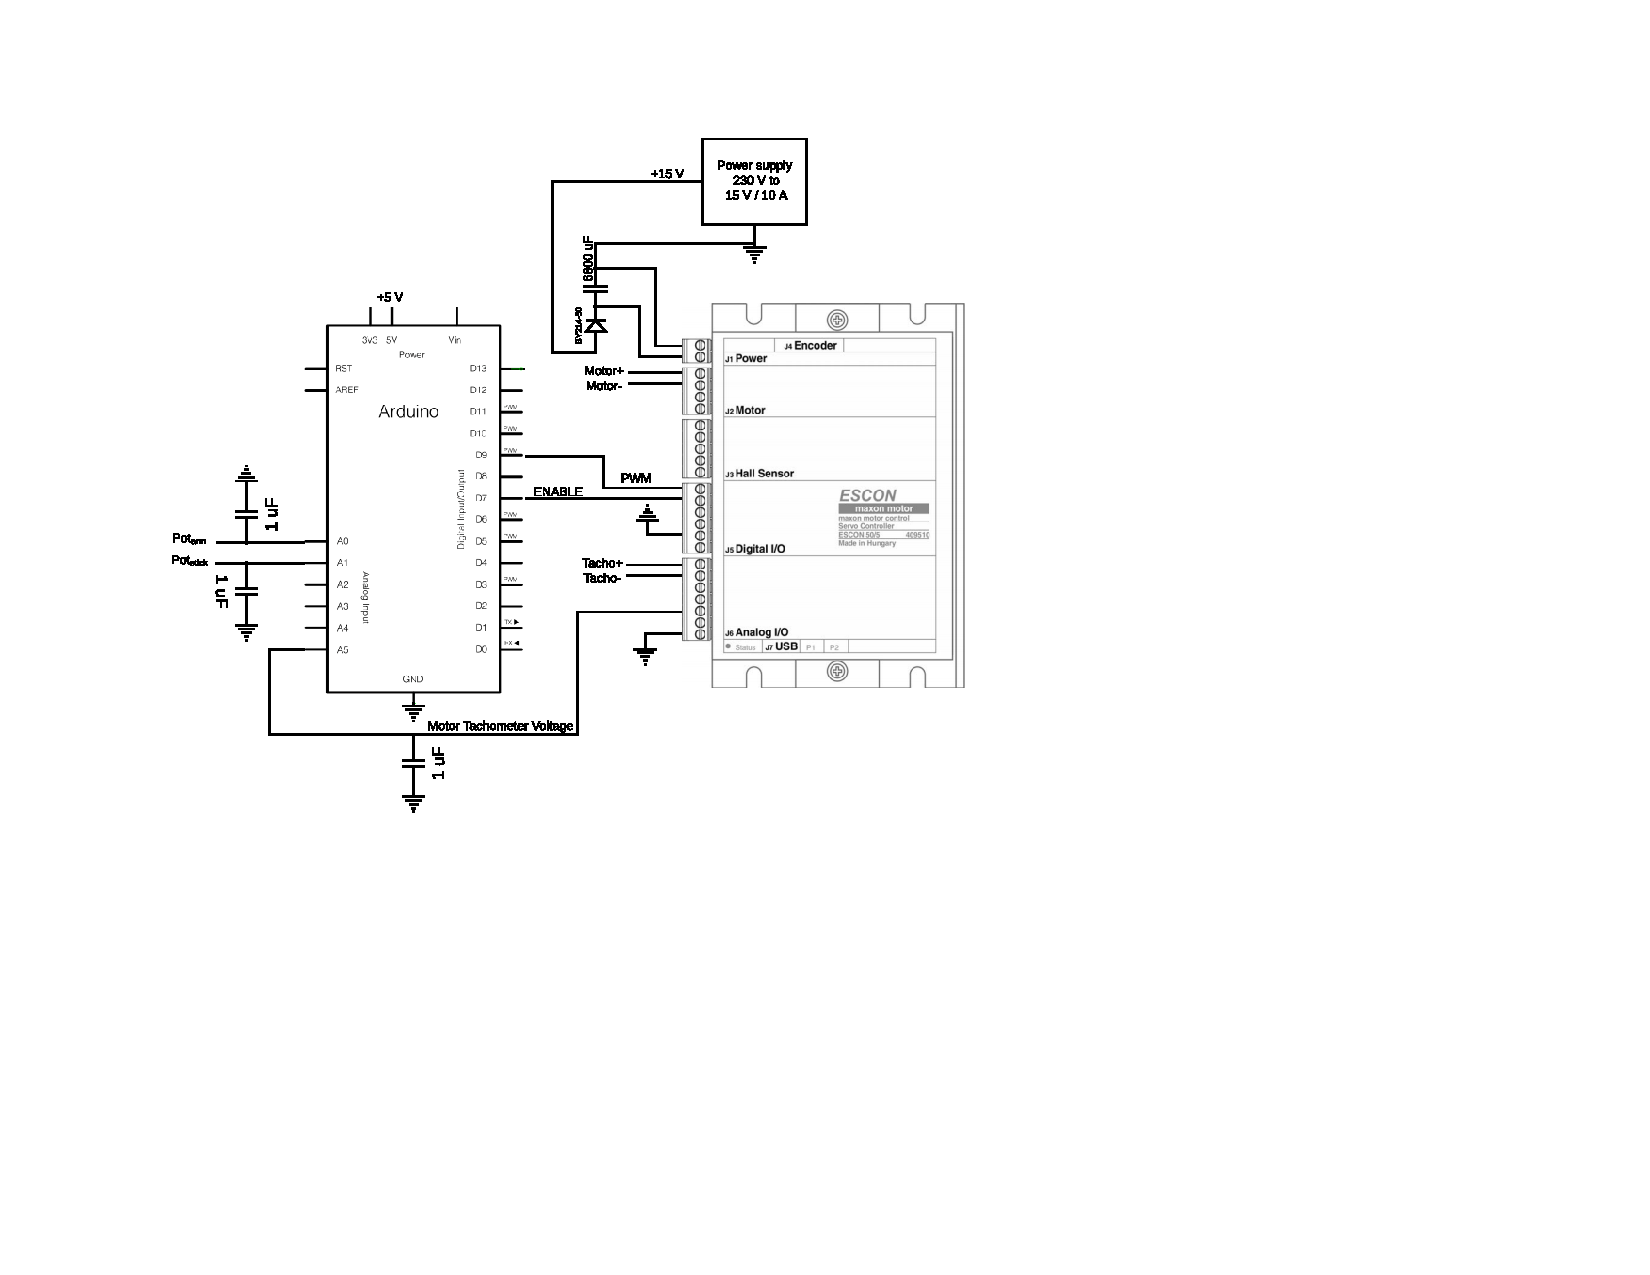
\includegraphics[width=0.85\linewidth]{figures/MotorControllerSetup}
\caption{Wiring for the control setup.}
\label{fig:EsconWiring}
\end{figure}
\newpage
The control PWM signal from the Arduino is set with a frequency of 5 kHz because that it is the maximum input frequency the motor controller will accept. It is set to 5 kHz so that the PWM avoids interference with the sampling frequency for the system.
The input PWM signal is then amplified and made faster. The output PWM frequency of the motor controller is 53,6 kHz with a duty cycle from 10 - 90\% which can not be changed in the ESCON studio. It is considered that the switching frequency of the ESCON is close to optimal when considering that the PWM frequencies is within the limit of what its datasheet specifies.   The main concern of a switching frequency of 53,6 kHz on the motor would be heat dissipation. Therefore the minimum PWM frequency for the motor is calculated to see if the motor controllers PWM frequency fits the motor.

\subsubsection{Calculating Minimum PWM Frequency}
The only PWM frequency considered is the minimum switching frequency for the motor. This is done by considering the motor resistance and inductance versus the maximum amount of current ripple wanted on the motor. The values for the resistance and the inductance of the motor are calculated in appendix \ref{tab_appendix:KeSetUp}. The formula is seen cf. \ref{eq:PWMSwitch} [Palle Andersen, 2016].

\begin{equation}
f_{switch} \geq \frac{-1}{2\cdot ln(1-\frac{p}{100})}\cdot\frac{R_{m}}{L_{m}}
\label{eq:PWMSwitch}
\end{equation}
Where:\\
\begin{tabular}{m{8em} m{25em} m{8em}}
$p$& The maximum \% current ripple in the motor. & [1]\\
$\frac{R_{m}}{L_{m}}$& The inverse electrical time constant of the motor.& [Hz]\\
\\
\end{tabular}

Replacing with the numerical values of the resistance and the inductance and choosing a max ripple percentage of 5\%, the minimum switching frequency determined to be:
\begin{equation}
    f_{switch} \geq \frac{-1}{2 \cdot ln(1-\frac{5}{100})}\cdot\frac{0,82\ \Omega}{156\cdot10^-6 \ \cdot \text{H}} \approx \ 51,2 \text{kHz}
\end{equation}

The maximum ripple in the motor is determined by making the ripple the unknown factor P$_{ripple}$ and setting the PWM frequency to the implemented 53,6 kHz.  

\begin{equation}
    53,6 \text{kHz} = \frac{-1}{2 \cdot ln(1-\frac{P_{ripple}}{100})}\cdot\frac{0,82\ \Omega}{156\cdot10^-6 \ \cdot \text{H}}\ =\ P_{ripple}\ = 4,785\%  
\end{equation}
This gives that the maximum current ripple is 4,785\% if considering a PWM frequency on 53,6 kHz. A general rule is that the ripple should be less than 10\% of the current, so considering that is less than 5\% is good considering that the system is implemented with current control.


%https://playground.arduino.cc/Code/Timer1
 
\subsection{Implementing Controllers}
The implementing on the hardware has been described in the chapter, and therefore the implementation can proceed to the implementing the controllers on an Arduino. 

\subsection{Implementing Continuous Controller on Arduino}
As the Arduino is a microprocessor the continuous controller found in \autoref{sec:IPController} needs to be transformed into a discrete controller. This also means a sample time needs to be determined. The sample time needs to be faster than the settling time of the fastest subsystem i.e. the motor loop. The motor loop has a settling time of 0.0137 seconds. The sample time is selected to be 0.002 seconds as it's faster than the motor loop. This gives a sampling frequency of \autoref{eq:ArduinoFs}.
\begin{flalign}
F_s=500\text{ Hz}\label{eq:ArduinoFs}
\end{flalign}

With the sampling time determined the continuous controller needs to be transformed to a discrete controller. For the two P-controllers it's as simple as multiplying the sampled input with the gain to get the discrete output. For the outer loop controller it's not as simple and is done by using the Z-transform. There are a couple of different options for performing the Z-transform each with their own nuances but the differences won't be discussed and the bilinear transform will be used. For the bilinear transform $s$ in \autoref{eq:outerLeadController} will be substituted with \autoref{eq:s=z}.
\begin{flalign}
s=2F_s\frac{z-1}{z+1}\label{eq:s=z}
\end{flalign}

\autoref{eq:outerLeadController} then becomes \autoref{eq:DxBilinear}.
\begin{subequations}\label{eq:DxBilinear}
\begin{flalign}
&D_x=8.8\frac{2F_s\frac{z-1}{z+1}+4.29}{2F_s\frac{z-1}{z+1}+9.19} \\
&D_x=8.8\frac{2F_s(z-1)+4.29(z+1)}{2F_s(z-1)+9.19(z+1)} \\
&D_x=8.8\frac{(2F_s+4.29)z+4.29-2F_S}{(2F_s+9.19)z+9.19-2F_s} \\
&D_x=\frac{Y(z)}{X(z)}=8.8\frac{2F_s+4.29+(4.29-2F_S)z^-1}{2F_s+9.19+(9.19-2F_s)z^-1} \\
&Y(z)\left(2F_s+9.19+(9.19-2F_s)z^-1\right)=8.8X(z)\left(2F_s+4.29+(4.29-2F_S)z^-1\right) 
\end{flalign}
\end{subequations}

The Z-transformed controller can then be made discrete by substituting $aY(z)z^m$ with $ay[k+m]$ and similarly for $X(z)$. This is gives the discrete controller ready to be implemented in the Arduino in \autoref{eq:DxDiscrete}.
\begin{subequations}
\begin{flalign}
&(2F_s+9.19)y[k]+(9.19-2F_s)y[k-1]=8.8(2F_s+4.29)x[k]+8.8(4.29-2F_S)x[k-1] \\
&y[k]=8.8\frac{2F_s+4.29}{2F_s+9.19}x[k]+8.8\frac{4.29-2F_S}{2F_s+9.19}x[k-1]-\frac{9.19-2F_s}{2F_s+9.19}y[k-1] \label{eq:DxDiscrete}
\end{flalign}
\end{subequations}



\subsubsection{Controller Software}
This sections describes the softwre implemented on the Arduino. 
\begin{figure}[htbp]
\centering
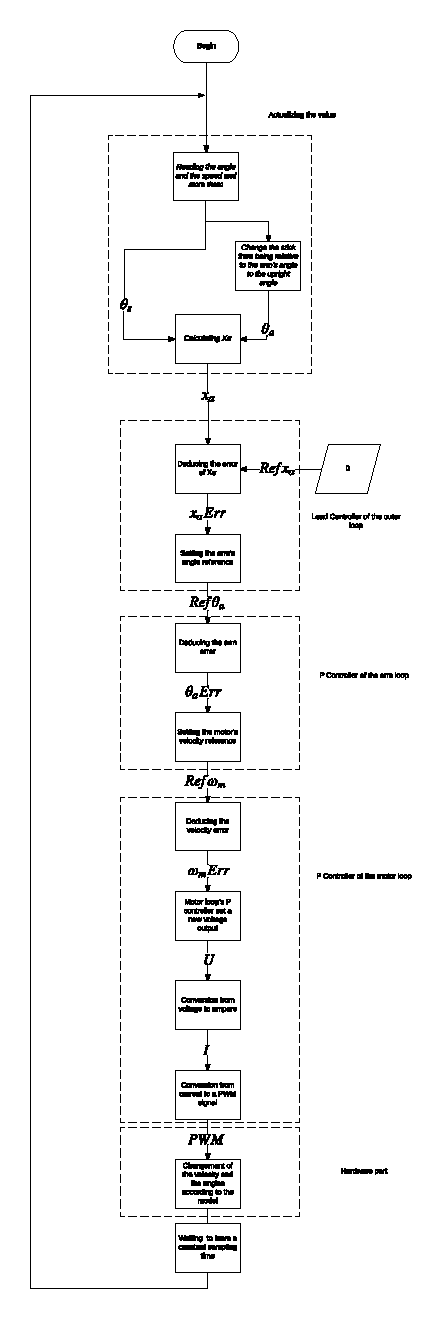
\includegraphics[width=1\linewidth]{figures/Flowchart.pdf}
\caption{Flowchart for the implemented software on Arduino.}
\label{fig:Flowchart}
\end{figure}
\newpage
\subsection{Implementation Evaluation}
This following sections describes the different problems that occurred with the hardware and software trough out the implementation. They will be explained to show the progress trough out the implementation.
\\
\subsubsection{Filtering Sensors}
During implementation of the Arm Loop it was found that a shaking occurred trough the motor, gear and out to the arm. From testing higher gains it was found that the shaking was amplified and became more unstable with the higher gains. Testing of the hardware and software was done to determine from where this shaking was sourced. To start with the sensors was checked for noise and floating. This was done to remove incorrect readings and unstable sensors. The sensors was read trough a oscilloscope and it was found that the ESCON motor controllers PWM frequency was represented in the sensor signal. This can occur from incorrect ground or wires not correctly isolated. This problem was solved by adding a capacitor to the sensors as seen cf. figure \ref{fig:EsconWiring}. The capacitor is connected from signal wires to ground to make a low pass filter. 1 $\upmu$F is chosen, one for each signal wire and considering that it is two 10 k$\Omega$ potentiometers it will give a varying cut of frequency. The cut-off frequency is calculated to:       

\begin{equation}
\frac{1}{2\cdot \pi \cdot 10000\ \Omega \cdot 1 \cdot 10^{-6}\  \text{F}}\ =\ 15,92\ \text{Hz}
\end{equation}

\begin{equation}
\frac{1}{2\cdot \pi \cdot 2,97\ \Omega \cdot 1 \cdot 10^{-6}\  \text{F}}\ =\ 53,6\ \text{Hz}
\end{equation}

Considering that the resistance changes we need to go under $\approx$ 2,97 $\Omega$ before the cut-off frequency exceeds the frequency of the noise, and that any resistance higher will dampen with more than -3 dB. It is noticeable that the resistance values of the potentiometers is in between both limits of resistances and the noise is therefore dampened. The conclusions of adding these filters removed high frequency noise that made the arm shake less. There was still a small-amplitude shaking around the setpoint when the arm was at a position and kept there. This could be down to bad range and bad optimisation of bits in the software. The software is made with scaling from analogue values down to radians, which means that reading the arm potentiometer and having a analogue value from 235 to 527 and converting it down to -0,785 to 0,785 radians will mean that that first two bits is not optimized, because they are static or close to. This gives that the 10-bit resolution of the PWM is not used optimally when two is static, but it is still better than having 8-bit with two static. This can be optimize by either changing the range of the potentiometers to that the radian range was optimized to cover from 0-1023 and have a better bit/radians resolution. This solution could be done by having a operational amplifier with a gain of 4 and a 5 V saturation. The potentiometer should then be turned to that -0,785 is at the 0 point for the potentiometer. It can also be solved by changing the model and with the conversion trough out the software. Meaning that the analogue value would not be converted which would give a better resolution for the PWM output. Equally they can be combined for the best resolution. It is chosen to only implement the resolution optimization if and only if the acceptance test show that the system does not fulfil the set requirements.

\subsubsection{PWM Frequency Problems}
The stick control loop was implemented. The simulations gave gains and results that could be implemented on the system. When implemented it was found that the arm did not control correctly when the stick moved. Repetitive test gave the conclusions that the speed of the arm was to slow. Higher gains was implemented but did not give the wanted result and the gains was set back to the simulated. A oscilloscope test was made on the Arduino PWM frequency by measuring the input frequency on the motor controller. The test showed that the frequency was 100 Hz and not 5 kHz as expected. The software was revised and determined that TimerOne was used as timer twice, one for controlling PWM frequency and one for controlling the sampling time with an interrupt. The interrupt was removed and changed to a wait so that the sampling time was kept constant. The PWM frequency was then measured to be 5 kHz and the arm then behaved as wanted with the simulated gains.    

\subsubsection{I2T Limitation}
Another problem observed where a run time limit on the control system. The system would slow down after around approximately a minut but it was easily observed trough the ESCON studio that a I2T limit was reached on the motor controller. An I2T limit is an algorithm that is described by the nominal current, the motor peak current in rms, and the motor peak current in seconds. It is used to secure the motor and driver from damage and over heating. The parameters for the algorithm was set trough the ESCON studio, with a nominal current on 5 A, a peak current on 11 A, and a thermal time constant on 200 seconds. When the limit is reached the motor current only goes to 5 A so the motor controller is shut off so that it cools down and can then be used again.  


\section{Rocket Implementation}

\subsection{Implementing Inertial Measurement Unit}

The system consists of an Inertial measurment Unit (IMU) GY - 80. This implies that multiple integreted sensors can be used, as seen in \autoref{sec:Rocket_sencor_choice}. The PCB created and used is seen in appendix \todo{appendix of PCB to do}. 
Mulitple physical and software constraints have to be taken into account when implementing the system.

The rise time and setling time of the sensors are an important feature when ensuring the stability of the rocket. It cannot be too slow, otherwise the system will react to late to any angle variation. The rise time and setling time of the servomotors and rocket transfer function are described in %\auto{tab:TableStepr}.
 The process of the servomotors is then considered fast enough for the system, not interfering with the angle control process.

The vibration of the rocket is a physical difficulty for the sensors as the measurements might be distorted. The placement and fixation must be carefully thought, as described in appendix \todo{appendix to do}.

Of all the sensors available, only the gyroscope will be used in this project. This is due to the conditions of the rocket launch : the rocket will be attached to the ground, and will therefore have no use of all the potential of the IMU GY -80.

\subsection*{Gyroscope}

The system includes a L3G4200D 3-axis gyroscope. The gyroscope is described in appendix \todo{appendix to do}. 

An example of implementing is done through a pseudo-code which converts in degree the output of the sensor in order to trace the rotation and mouvement of the system. The angle are then analyzed to measure the angle variation, and then enable the system to correct the variation.

\subsection{Test of simulated flight}

The system is connected to the servomotors. The goal is to simulate manually an angle variation of the rocket body and see the reaction of the system on the servomotors and the thruster. If the real thruster angle is equal to the desired one, then the controller is deemed acceptable and the system as fullfilling the requirements.

The expirement set up is described in appendix \todo{appendix to do}. An example of implementing is done through 
\todo{do the code/expirement to finish that part}.

\subsection{Test of attached-rocket flight}

The expirement set up is described in appendix . 